\begin{abstract}
Caching an agent step can change a downstream decision even when repeated calls to that step appear identical. We study this gap using frozen executions of synthetic procurement workflows with nondeterministic language-model steps and a deterministic approve/reject/escalate consumer. A recorded Gemma3 chain produces identical validated outputs on 260 configured temperature-zero same-prompt pairs for each feeding step, yet declared dependency reuse introduces two unsafe approvals on one request: a stable but wrong justification changes on a perturbed prompt that the declaration treats as irrelevant. We then evaluate a policy-specific decision-equivalence certificate using structured request differences, cached candidate outputs, fresh noncandidate outputs, and finite valid-output witnesses. Across three chain configurations it certifies 82.1--85.3\% of recorded perturbations and saves 50.5--52.1\% of nominal feeding-step call slots, with zero decision changes on certified, scoreable cases. One DeepSeek and 30 Phi4-mini rows are unscoreable; they remain in fraction denominators and receive no equivalence guarantee. The results distinguish observed repeatability, correctness, and consumer equivalence, and provide a reproducible offline test rather than a deployed reuse runtime.
\end{abstract}
\maketitle
\iflongversion
\noindent\textit{Empirical preprint; not peer reviewed. 6 October 2026.}
\fi

\section{Introduction}
An agent workflow often uses a language model to construct a record, then applies ordinary code to decide what to do. Reusing the model's record can avoid another inference call. Whether that reuse preserves behavior depends on the code that consumes the record, the fields that may change, and the distinction between a correct result and a repeatable one.

Existing systems provide several relevant mechanisms. LangGraph caches node results by an input-derived key~\cite{langgraph}. VisTrails explicitly assumes that cacheable modules produce the same outputs for the same inputs, and permits nondeterministic modules to be marked non-cacheable~\cite{vistrails}. Temporal addresses durable execution by placing nondeterministic operations, including LLM invocations, in Activities outside the workflow replay path~\cite{temporal}. These mechanisms do not assert that a cached interpretation remains equivalent to a fresh interpretation after another part of its prompt changes.

We investigate that narrower question through \systemname{}, an offline study of recorded agent executions. Our contribution is an empirical counterexample and a bounded certificate experiment. In the counterexample, both feeding steps match on every configured temperature-zero same-prompt comparison (260 pairs per step). A field-level dependency declaration nevertheless reuses a consistently wrong, decision-relevant output while a fresh call corrects it. Two reuse-induced approvals cross a synthetic policy boundary. This shows why same-prompt repeatability alone cannot validate a dependency declaration.

The certificate experiment moves the check to the deterministic consumer. It asks whether all enumerated valid outputs of the reuse candidates lead to the same decision, with fresh outputs of other steps and authoritative request fields fixed. This criterion permits reuse even when the candidates themselves vary, and rejects a repeatable output when alternatives can change the decision. We report its coverage, nominal call-slot savings, disagreements, and invalid-output exclusions on three frozen chain sweeps. All six intended sweeps, the original model responses, policy code, number generators, and figure inputs accompany the analysis. The measured benefit is avoiding counterfactual feeding-step slots; execution latency, certificate overhead, and deployment safety remain unmeasured.

\section{Workload and measurement}
\label{sec:workload}
\paragraph{A deterministic consumer.}
The workload consists of 65 synthetic procurement requests generated with seed 42. Each includes planted structured truth and rendered prose. The consumer returns one of \texttt{approve}, \texttt{reject}, or \texttt{escalate}; it does not execute a purchase. Supplier sanctions or lack of approval cause rejection. Compliance gaps, supplier risk, unknown categories, over-budget purchases, and amounts exceeding a category ceiling cause escalation. A confidence gate also escalates purchases close to the binding ceiling. Invalid structured outputs fail validation and escalate.

The two-step workflows compare an LLM interpreting request and supplier fields (A2) with a version in which three supplier fields come from an authoritative record (A3). In both, deterministic code decides and a later LLM explains the decision. The chain (C3) adds a separate justification interpreter. It produces eight model-derived fields in total: six request fields from \texttt{parse} and two justification fields from \texttt{justify}. Three supplier fields remain authoritative. Both feeding prompts contain the request prose; they declare different output fields, but prompt dependence need not respect that partition. The explanation is a sink and cannot alter the decision (Figure~\ref{fig:architecture}).

\begin{figure*}[t]
\centering
\begin{tikzpicture}[x=1.95cm,y=1cm,>=Stealth,
  box/.style={draw,rounded corners=1pt,align=center,font=\fontsize{8}{9}\selectfont,minimum height=.6cm,inner sep=3pt},
  arr/.style={->,line width=.5pt}]
\node[box,text width=1.9cm] (r) at (0,1.8) {Synthetic\\request};
\node[box,text width=2.0cm] (p) at (1.65,2.4) {Parse LLM\\6 fields};
\node[box,text width=2.0cm] (j) at (1.65,1.2) {Justify LLM\\2 fields};
\node[box,text width=2.0cm] (v) at (3.4,1.8) {Validate\\and merge};
\node[box,text width=1.9cm] (d) at (5.1,1.8) {Policy\\decision};
\node[box,text width=1.8cm] (e) at (6.75,1.8) {Explain LLM\\sink};
\node[font=\fontsize{8}{9}\selectfont,align=center] (s) at (3.4,3.15) {Authoritative supplier fields};
\draw[arr] (r) -- (p); \draw[arr] (r) -- (j);
\draw[arr] (p) -- (v); \draw[arr] (j) -- (v);
\draw[arr] (s) -- (v); \draw[arr] (v) -- (d); \draw[arr] (d) -- (e);
\node[box,text width=4.0cm] (obs) at (1.05,-.25) {Structured request diff;\\canonical candidates;\\fresh noncandidate outputs};
\node[box,text width=3.3cm] (w) at (3.6,-.25) {Enumerate valid\\candidate witnesses};
\node[box,text width=3.7cm] (g) at (6.05,-.25) {Consumer decisions constant?\\Certify reuse;\\otherwise recompute};
\draw[arr] (obs) -- (w); \draw[arr] (w) -- (g);
\draw[densely dashed] (-.65,.8) -- (7.3,.8);
\node[font=\fontsize{8}{9}\selectfont,anchor=west] at (-.6,.55) {Offline certificate analysis of recorded executions};
\end{tikzpicture}

\caption{Measured chain and offline certificate boundary. Both feeding steps read the request independently; validation can stop execution before later steps. The lower path analyzes recorded outputs and does not constitute an implemented serving runtime. Evaluation-only oracle decisions and perturbation labels are outside the certificate's inputs.}
\Description{A synthetic request feeds parse and justify language-model steps; their validated fields merge with authoritative supplier fields into a deterministic policy decision and a final explanation. A separate offline path receives a structured request difference, canonical candidates, and fresh noncandidate outputs, enumerates candidate witnesses, and checks constant consumer decisions.}
\label{fig:architecture}
\end{figure*}

The chain consumer adds a justification rule: after earlier rejection and escalation rules, an amount at least 25\% of the binding ceiling escalates if the justification is inadequate. The binding ceiling is the smaller of remaining budget and the category limit. Adequacy is therefore decision-relevant only on some records. Urgency and justification category are validated but do not affect this fixed policy. The seed realizes 34 inadequate justifications; the rule fires on five canonical ground-truth requests and changes four decisions relative to the earlier consumer. These figures describe deliberate workload construction, not a procurement population.

\paragraph{Six frozen sweeps.}
Three two-step configurations use \texttt{deepseek-\allowbreak chat}, \texttt{deepseek-\allowbreak reasoner}, and \texttt{gemma3:4b}; three chain configurations use \texttt{deepseek-\allowbreak chat}, \texttt{gemma3:4b}, and \texttt{phi4-mini}. Each starts from the same 65 seed-generated base requests. Canonical and perturbation calls are configured at temperature zero; ten repeated runs per request use configured temperature 0.7 to expose variation. The thinking endpoint does not honor temperature in the same way: current provider documentation states that temperature has no effect in thinking mode~\cite{deepseek}. Thus these are recorded configuration labels, not controlled comparisons of sampling temperature. Main sweeps were collected in July 2026, chain sweeps in September; model aliases and collection dates confound comparisons across them.

The chain E8 analysis requires valid canonical outputs for both feeding steps: 65 DeepSeek, 65 Gemma3, and 59 Phi4-mini base requests qualify. Six Phi4-mini canonical failures are skipped before its 935 perturbation rows are analyzed; DeepSeek and Gemma3 each contribute 1,029 rows. Skipping them does not make the original 65-request sweep disappear from provenance.

\paragraph{Three different observations.}
We distinguish \emph{observed repeatability}, equality of validated output fields on recorded calls with the same prompt; \emph{correctness}, agreement with planted request truth; and \emph{decision equivalence}, agreement of downstream decisions. We call a consumer an \emph{absorber} on a measured set when its input parse states vary while its decision remains unchanged; such states may include validation failure. Absorption is scoped to that consumer and set, and can occur around an incorrect constant decision. No finite comparison establishes that an LLM is a mathematical function.

For reuse, the reference decision is the recorded fresh execution on the perturbed request. A \emph{decision change} is disagreement with this reference. A \emph{reuse-induced unsafe approval} additionally requires that reuse approves while the planted-truth oracle does not approve. This narrower count excludes errors shared by fresh execution and reuse; zero such errors does not imply oracle correctness. The oracle applies the same consumer to ground-truth fields and is available for evaluation only.

\iflongversion
\subsection{Collection and corpus accounting}
Table~\ref{tab:sweeps} lists the retained configurations. The main runs compare four architectural variants: direct LLM decisions, LLM decisions given a precomputed policy report, deterministic decisions on LLM-parsed records (A2), and deterministic decisions with authoritative supplier fields (A3). The chain C3 splits request parsing and justification into distinct validated outputs. The present analysis centers on A2/A3 and C3; other variants remain reproducible context rather than evidence of a universal architectural ranking.

\begin{table}[t]
\centering\small
\begin{tabular}{lll}
\toprule
Workflow & Recorded model & Collection \\
\midrule
Two-step & \texttt{deepseek-\allowbreak chat} & 18 July 2026 \\
Two-step & \texttt{deepseek-\allowbreak reasoner} & 18 July 2026 \\
Two-step & \texttt{gemma3:4b} & 22 July 2026 \\
Chain & \texttt{deepseek-\allowbreak chat} & 3 Sept. 2026 \\
Chain & \texttt{gemma3:4b} & 3 Sept. 2026 \\
Chain & \texttt{phi4-mini} & 3--4 Sept. 2026 \\
\bottomrule
\end{tabular}
\caption{Six intended frozen sweeps, each with 65 base requests and seed 42. Model aliases identify recorded calls and are not immutable provider snapshots.}
\label{tab:sweeps}
\end{table}

The artifact retains available call specifications, raw responses, parsed fields, schema-validity flags, canonical records, repeated samples, and perturbation rows. Some legacy cache records lack stored prompts; complete prompt storage is not asserted for every sweep. The replay analysis reads those files and performs no new model calls. Perturbations change request amount, category, budget, urgency, compliance fields, supplier attributes, or justification. They are finite, policy-directed contrasts around the same base requests, not independent requests sampled from a deployment distribution.

For all three headline chain configurations, same-prompt tests compare canonical outputs with recorded temperature-zero calls, and exact stored-prompt comparisons verify that supplier-side perturbations leave the prompts unchanged. One legacy main A3 comparison, DeepSeek Chat, records prompt identity by construction rather than complete stored-prompt verification. Their canonical records are reused across comparisons, so pairs are clustered by request. Ten repeated samples used for absorption are a separate measurement.

\subsection{Variation can be absorbed without establishing reuse}
Table~\ref{tab:absorption} illustrates the distinction in the main sweeps. Its denominator for absorption is the number of requests with varying parse states across repeated samples; each state is a validated field record or an invalid-parse marker. Decision variation uses all 65 requests. For A3, DeepSeek Chat absorbs nine of ten varying requests, DeepSeek Reasoner 20 of 23, and Gemma3 all five. The varying sets include invalid-bearing requests: one Chat A2, four Gemma3 A2, and one Gemma3 A3 request contain invalid samples. These observations concern the particular consumer and sampled states. They do not establish that any other prompt, field substitution, or consumer will preserve a decision.

\begin{table}[t]
\centering\small
\begin{tabular}{llrrr}
\toprule
Model & Variant & Varying & Absorbed & Decisions vary \\
\midrule
Chat & A2 & \absFlagAtwoEoneParseVarN & \absFlagAtwoEoneAbsorbed & \absFlagAtwoEoneDecVar \\
Chat & A3 & \absFlagAthreeEoneParseVarN & \absFlagAthreeEoneAbsorbed & \absFlagAthreeEoneDecVar \\
Reasoner & A2 & \absThinkAtwoEoneParseVarN & \absThinkAtwoEoneAbsorbed & \absThinkAtwoEoneDecVar \\
Reasoner & A3 & \absThinkAthreeEoneParseVarN & \absThinkAthreeEoneAbsorbed & \absThinkAthreeEoneDecVar \\
Gemma3 & A2 & \absLocalAtwoEoneParseVarN & \absLocalAtwoEoneAbsorbed & \absLocalAtwoEoneDecVar \\
Gemma3 & A3 & \absLocalAthreeEoneParseVarN & \absLocalAthreeEoneAbsorbed & \absLocalAthreeEoneDecVar \\
\bottomrule
\end{tabular}
\caption{Repeated-sample absorption in the two-step workflows. \emph{Varying} and \emph{absorbed} count requests, including changes to or from the invalid-parse marker; the last column is the fraction of all 65 requests with decision variation. No row is an estimate of general cache correctness.}
\label{tab:absorption}
\end{table}
\fi

\section{A reuse counterexample}
\label{sec:counterexample}
We compare full recomputation with a declared dependency rule. A feeding step is a reuse candidate when no changed structured request field intersects its declared output fields. This declaration permits \texttt{justify} reuse after a request-side change such as urgency, even though the step still reads the changed prose. An exact-input key is a more conservative comparator; oracle-labelled irrelevance is retained as an evaluation diagnostic, not a realizable runtime policy.

The Gemma3 chain matches validated records on all \absChainGmParseEtwoRecPairs{} configured temperature-zero same-prompt pairs for \texttt{parse} and all \absChainGmJustifyEtwoRecPairs{} for \texttt{justify}; these pairs have exactly matching stored prompts. Declared dependency reuse still introduces \absChainGmEthreePtwoUnsafe{} unsafe approvals and \absChainGmEthreePtwoDivN{} decision changes on one request. The DeepSeek chain produces one decision change without a reuse-induced unsafe approval; Phi4-mini produces none on scoreable rows. Their dependency rule admits roughly the same nominal reuse opportunities by construction, so its coverage is not a model-quality measure.

The separating Gemma3 request is \texttt{req-008-\allowbreak clean\_\allowbreak approve}. Its canonical justification adequacy is wrong relative to planted truth and stable across the repeated samples used in the field decomposition. Altering that field can change the consumer's decision: it is \emph{load-bearing}. On two urgency perturbations, a fresh justification changes the adequacy field and the fresh workflow escalates, while reuse retains the wrong adequate justification and approves. Across all 14 rows where this justification is a declared reuse candidate, its fresh output changes on four. A different request has a stable, wrong, load-bearing category, but its fresh category never changes on its five candidate rows and produces no corresponding reuse break. Stability, wrongness, and load-bearing status explain the failure mechanism; all three alone are insufficient without a relevant fresh-output change.

The declaration conflates a step's output schema with its prompt dependencies. The observation does not refute deterministic memoization under an actual complete input key, or recorded replay of a previous Activity. It shows that measured same-prompt equality does not license reuse across a changed prompt, even when the changed field is absent from the step's declared outputs.

\section{Checking the consumer before reuse}
\label{sec:certificate}
The E8 experiment adds a certificate to the declared reuse candidates. Let $J$ be the candidate feeding steps and $z$ the assembled record using canonical outputs for $J$, fresh validated outputs for noncandidates, and the perturbed request's authoritative supplier fields. Let $W_J(z)$ be the implemented joint set of valid-output witnesses for the candidates. With deterministic consumer $D$, the equivalence check is
\begin{equation}
\operatorname{cert\_eq}(z,J)\;\Longleftrightarrow\;
 \{D(w):w\in W_J(z)\}=\{D(z)\}.
\label{eq:certificate}
\end{equation}
On acceptance, the analysis substitutes the canonical candidate outputs; otherwise it uses recorded recomputation. Acceptance certifies constancy over this implemented witness set. It is independent of whether the canonical candidates equal the ground truth.

\paragraph{What the certificate observes.}
Candidates are computed from a field-wise diff between structured base and perturbed requests. The certificate uses cached canonical outputs and fresh noncandidate outputs; it does not need the fresh candidate's contents for its decision. Oracle decisions, perturbation-factor labels, and precomputed oracle sensitivity are reserved for scoring. A guarded test raises if the certificate reads those evaluation-only inputs. The present workload exposes structured differences directly. Recovering reliable differences from unrestricted prose is a separate deployment problem.

\paragraph{What it enumerates.}
Booleans and categories have finite witnesses. Amount and budget witnesses lie at comparison cuts, between cuts, at zero, and beyond the largest cut. The cuts derive from budget, category ceiling, and the fixed 0.25 and 0.9 shares of the binding threshold. When a whole parse step is a candidate, the implementation enumerates category, compliance booleans, representative budget regimes, and corresponding amount cuts jointly; a candidate justification varies adequacy. Decision-inert urgency and justification category retain one witness. The certificate is specialized procedural enumeration for this straight-line policy and nonnegative finite values. Tests check its boundaries and information restrictions; the experiment supplies no general proof for arbitrary policies, numeric programs, or LLM output spaces.

\paragraph{Invalid outputs are outside the equivalence check.}
The consumer escalates invalid input, but the equivalence check enumerates valid classes. If a fresh noncandidate output is invalid or missing, the analysis cannot assemble a scored record and marks the row unscoreable. There are \absChainGmEeightUnscoreable{} such Gemma3 rows, \absChainDsEeightUnscoreable{} DeepSeek row, and \absChainPhEeightUnscoreable{} Phi4-mini rows; three Phi4-mini rows also have an invalid fresh candidate. Early parse failure can prevent the later justification call from occurring. These rows are explicitly excluded from decision-disagreement scoring. Consequently zero scored changes provides no guarantee about accepting reuse when a counterfactual fresh candidate would be invalid.

\section{Certificate results and tradeoffs}
\label{sec:results}
\begin{figure*}[t]
\centering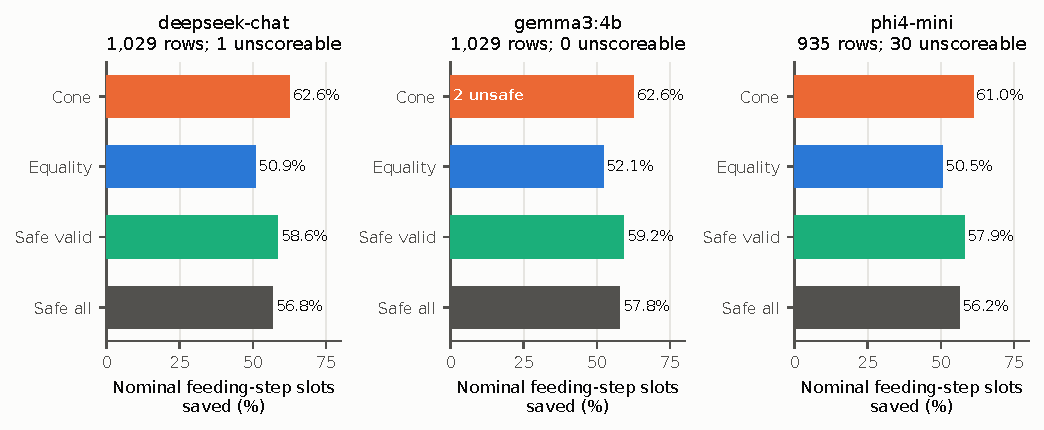
\includegraphics[width=\textwidth]{../../publication/figures/certificate-tradeoff.pdf}
\caption{Declared-cone baseline and E8 guards on the three frozen chain configurations. The horizontal axis is nominal feeding-step slot savings, divided by two slots per row including unscoreable rows. Equality is the primary criterion. Approval-oriented guards permit conservative changes; zero scored unsafe approvals does not cover invalid fresh outputs or establish a deployment guarantee.}
\Description{Three panels compare nominal feeding-step slot savings under declared-cone reuse, equivalence, safety over valid witnesses, and safety including an invalid-output class for DeepSeek, Gemma3, and Phi4-mini. The Gemma3 declared-cone bar marks two recorded unsafe approvals; certified coverage is reported separately in tables.}
\label{fig:tradeoff}
\end{figure*}
\begin{table}[t]
\centering\small
\setlength{\tabcolsep}{3pt}
\resizebox{\columnwidth}{!}{% Generated primary cert_eq table. Invalid/excluded rows remain in fraction denominators.
\begin{tabular}{lrrrrrr}
\toprule
Model & Rows & Excluded & Certified & Saved slots & Changes & Unsafe \\
\midrule
DeepSeek & 1{,}029 & 1 & 852 & 50.9\% & 0 & 0 \\
Gemma3 & 1{,}029 & 0 & 878 & 52.1\% & 0 & 0 \\
Phi4-mini & 935 & 30 & 768 & 50.5\% & 0 & 0 \\
\bottomrule
\end{tabular}
}
\caption{E8 \texttt{cert\_eq}. Excluded rows are unscoreable. Certified counts use all rows as their fraction denominator; savings use two nominal feeding-step slots per row. Changes and reuse-induced unsafe approvals are scored only where a complete valid fresh record exists.}
\label{tab:certificate}
\end{table}

Table~\ref{tab:certificate} reports \texttt{cert\_eq} on the frozen chain sweeps. It certifies \absChainDsEeightCertifiedN/\absChainDsEeightRows{} DeepSeek rows (\absChainDsEeightCertifiedPct), \absChainGmEeightCertifiedN/\absChainGmEeightRows{} Gemma3 rows (\absChainGmEeightCertifiedPct), and \absChainPhEeightCertifiedN/\absChainPhEeightRows{} Phi4-mini rows (\absChainPhEeightCertifiedPct). The corresponding nominal feeding-step slot savings are \absChainDsEeightSavedPct, \absChainGmEeightSavedPct, and \absChainPhEeightSavedPct. No certified scoreable row changes the decision or introduces an unsafe approval. The two Gemma3 counterexample rows fail the equivalence check.

Certified fractions retain every E8 row in their denominator, including unscoreable rows. Savings count candidate steps reused, divided by $2R$ for $R$ recorded rows. This is an offline counterfactual over two feeding-step slots per row, including slots that fail-fast execution might never call. The numerators are \absChainDsEeightSavedN, \absChainGmEeightSavedN, and \absChainPhEeightSavedN; they are not measured API bills, end-to-end call reductions, or runtime speedups. The \absChainDsEeightScoreable, \absChainGmEeightScoreable, and \absChainPhEeightScoreable{} valid fresh records are the scoring subsets.

Two approval-oriented guards expose a coverage-versus-equivalence tradeoff (Figure~\ref{fig:tradeoff}). \texttt{cert\_\allowbreak safe\_\allowbreak valid} permits conservative decision changes but rejects an approving reuse if any enumerated valid candidate output would not approve. \texttt{cert\_\allowbreak safe\_\allowbreak all} also accounts for an invalid-output class, which always escalates; therefore an approving reuse cannot satisfy it. It reduces to accepting a recorded non-approval. In these sweeps, these guards save more nominal slots than equivalence, but each changes one scored DeepSeek decision; both changes are conservative, with no reuse-induced unsafe approval. Their zero unsafe counts remain finite-corpus observations.



\iflongversion
\subsection{Reading the certificate boundary}
Equation~\ref{eq:certificate} deliberately asks about the consumer, not about reconstructing an LLM distribution. For example, a sanctioned supplier causes rejection before most model-derived fields are consulted. Varying a candidate's valid request interpretation can then leave the decision fixed, making reuse possible without asserting that interpretation is correct. Near an approval boundary, however, an alternative justification or amount can trigger escalation and block equality. This policy structure explains why a guard can reject the repeatable Gemma3 error while accepting many other records.

The retained witness implementation is compact enough to inspect. Six known categories plus an unknown-category witness cover distinct ceiling behavior. For a parse candidate, each known category uses budget representatives of zero, half the category ceiling, and twice that ceiling. Compliance booleans vary jointly. Amount witnesses include the budget, category ceiling, and 0.25 and 0.9 times their minimum, with points on either side represented by interval witnesses. For a justification candidate, adequacy varies over both Boolean values. When both steps are candidates, the analysis takes their product. The artifact also checks field-wise amount and budget boundary behavior. This is evidence about the implemented finite policy quotient; changing the policy or schema requires revisiting its witnesses and tests.

The invalid path is materially different. A parse failure can leave no fresh justification output. Replacing the invalid parse with a cached record would then require a justification that the historical trace never produced. E8 does not synthesize this missing output, mark the row safe, or count it as an equivalence success. Its retained certification and slot-count denominator conventions include all rows, while scored disagreements exclude incomplete records. The distinction prevents the artifact's percentages from being read as correctness over every recorded execution.

\begin{table*}[t]
\centering\small
% Generated E8 table. Certified fraction uses ALL rows; saved slots use 2*ALL rows.
\begin{tabular}{llrrrr}
\toprule
Model & Scheme & Certified & Saved slots & Changes & Unsafe \\
\midrule
DeepSeek & cert\_eq & 82.8\% & 50.9\% & 0 & 0 \\
DeepSeek & cert\_safe\_valid & 93.8\% & 58.6\% & 1 & 0 \\
DeepSeek & cert\_safe\_all & 90.2\% & 56.8\% & 1 & 0 \\
Gemma3 & cert\_eq & 85.3\% & 52.1\% & 0 & 0 \\
Gemma3 & cert\_safe\_valid & 94.9\% & 59.2\% & 0 & 0 \\
Gemma3 & cert\_safe\_all & 92.0\% & 57.8\% & 0 & 0 \\
Phi4-mini & cert\_eq & 82.1\% & 50.5\% & 0 & 0 \\
Phi4-mini & cert\_safe\_valid & 92.2\% & 57.9\% & 0 & 0 \\
Phi4-mini & cert\_safe\_all & 88.8\% & 56.2\% & 0 & 0 \\
\bottomrule
\end{tabular}

\caption{All retained E8 schemes. \emph{Saved slots} denotes nominal feeding-step slots. Certified fractions include unscoreable rows; changes and reuse-induced unsafe approvals use the scoreable subsets specified in the text. Safety means the implemented approval-oriented criterion, not oracle correctness of all decisions.}
\label{tab:allguards}
\end{table*}
\fi

\section{Canaries measure a different question}
\label{sec:canary}
Rerunning a sample of cached requests can reveal disagreement, but this detects observed instability rather than validating a dependency declaration. We compute a finite-population model from same-prompt pairs. For request $i$, let $p_i$ be its observed mismatch fraction. If $k$ distinct requests are sampled uniformly without replacement, and fresh comparisons are conditionally independent with those fixed probabilities, modeled detection is
\begin{equation}
D(k)=1-\frac{1}{\binom{N}{k}}
 \sum_{\substack{S\subseteq\{1,\ldots,N\}\\|S|=k}}
 \prod_{i\in S}(1-p_i).
\label{eq:canary}
\end{equation}
The artifact evaluates this expression by dynamic programming. The resulting detection values are model calculations, not observed deployment probabilities. They assume neither provider drift nor temporal correlation, and plug in sparse measured fractions without estimating their uncertainty.

\iflongversion
\begin{figure*}[t]
\centering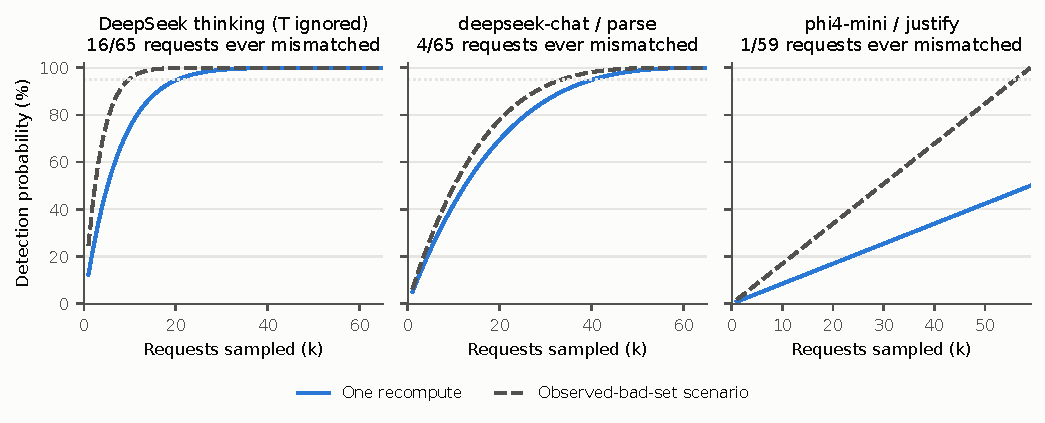
\includegraphics[width=\textwidth]{../../publication/figures/canary-detection.pdf}
\caption{Modeled detection of same-prompt output disagreement under Equation~\ref{eq:canary}. Curves use request-level sampling without replacement and plug-in mismatch fractions; the upper scenario treats each request with an observed mismatch as certain to mismatch. This scenario is not a confidence bound. Canaries do not detect stable wrong outputs or prove changed-prompt reuse safe.}
\Description{Three panels show detection as a function of sampled requests for DeepSeek Reasoner A3, DeepSeek chain parse, and Phi4-mini chain justify, using measured mismatch fractions and a scenario with certainty at observed mismatching requests.}
\label{fig:canary}
\end{figure*}
\fi

The reasoner A3 reaches modeled 95\% detection at \absThinkAthreeCanaryK{} of 65 requests; DeepSeek chain parsing at \absChainDsParseCanaryK{} of 65. Phi4-mini justification has one mismatching request among 59 eligible requests and an observed probability of one half on that request, so its plug-in ceiling is \absChainPhJustifyCanaryCeiling{} even when all are sampled. Conversely the Gemma3 same-prompt pairs have zero observed mismatches: this model predicts no detections, yet the changed-prompt counterexample remains. A zero-mismatch curve is evidence of the model's scope, not a safety certificate.

\section{Related work and scope}
Semantic response caching already trades input similarity against cache errors. GPTCache evaluates incorrect hits and explicitly discusses their cost~\cite{gptcache}; we do not assume that earlier semantic caches ignore false positives. Mnimi addresses the statistical independence of cached samples in probabilistic LLM workflows~\cite{mnimi}. StepCache verifies and selectively regenerates reusable output steps with task-aware checks~\cite{stepcache}. These establish that LLM reuse and verification are existing topics. Our experiment contributes a concrete repeatability-versus-reuse separation and consumer-equivalence measurement for a fixed structured policy. It neither benchmarks against these systems nor claims a general first reuse mechanism.

The principal limitation is the workload: one synthetic policy, one seed, finite perturbations, and six recorded configurations. Corpus choices deliberately exercise policy boundaries, and absolute disagreement rates cannot be extrapolated to real procurement or arbitrary agent tasks. No fresh release-time model calls were made, so provider changes cannot be separated from architecture or chronology. The repeatability pairs share canonical records; they do not provide independent Bernoulli trials. The certificate requires complete structured differences and a small deterministic consumer, and its computation and integration costs are not measured. Fresh invalid candidates remain outside its valid-output guarantee.

\iflongversion
\subsection{Reproduction and further experiments}
The accompanying publication artifact at \url{https://github.com/landigf/publication-artifacts/tree/main/Absorbers} preserves the six frozen sweeps and records input and generated-result checksums. Its pinned environment reruns validations, E1--E3 analysis, E8 field decomposition and certificates, number generation, and the publication figures without provider credentials or online inference. The numerical tables and curves in this manuscript come from the generated publication reports, not manually transcribed chart values. Historical drafts and result files are retained separately from publication entrypoints.

A clean reproduction verifies request counts, seed consistency, canonical eligibility, raw-response references, policy hashes, certificate input restrictions, and unchanged result hashes. The intended reproduction target is the published frozen-data analysis. Recollecting a sweep against the same mutable provider alias is a new experiment and need not reproduce these model outputs. Artifact provenance supports independent checking of this distinction.

Further evaluation should vary seeds, policy shape, justification share, and prompt formulations, and compare complete input keys against learned dependency declarations. A serving implementation would need to version its policy and witnesses, recover structured diffs, handle invalid and missing outputs explicitly, and measure certificate overhead against actual skipped calls. A broader certificate claim would require an independently justified coverage argument for the consumer's entire admissible input domain. These are open requirements, not evidence already supplied by the present experiment.
\fi

\FloatBarrier
\section{Conclusion}
The measured Gemma3 chain separates observed same-prompt equality from safe changed-prompt reuse. A stable, wrong output becomes consequential when another prompt field changes a fresh interpretation. Checking the deterministic consumer's decision over implemented valid-output witnesses rejects those two reuse-induced approvals while retaining about half of nominal feeding-step slots in three frozen configurations. Invalid-output exclusions, finite witness scope, and unmeasured execution cost delimit that result. The practical next question is how to establish consumer equivalence with reliable dependencies and acceptable overhead in a live workflow.

\paragraph{AI assistance.}
Generative AI tools provided substantial assistance with analysis, code changes, literature checking, manuscript drafting, figures, and verification for this version. The artifact records automated checks and independent technical reviews. Submission and responsibility for the content remain with the human author.
\label{sec:body-end}
